% **************************************************
%   Wichtig für die verwendung der hsrmreport-Klasse!
%   
%   Die Datei hsrmreport.cls muss in dem selben Ordner sein
%   wie die .tex Datei die diese Klasse verwenden möchte.
%
%   Desweiteren ist die Dokumentenklasse nach aktuellem 
%   noch ohnen Optionen, sprich Zweiseitig, änderung 
%   der Schriftgröße oder ähnliches. Ich werde versuchen 
%   diese Features hinzu zufügen sobald es mir möglich ist. 
%
%   Falls Ihr Probleme, Anregungen oder Verbesserungen habt,
%   könnt ihr mir das gerne mitteilenen.
%
%   Es kann sein das ihr evtl. manche Packete noch installieren 
%   müsst bevor die Klasse Fehlerfrei funktioniert.
%   Meldungen wie "Command terminated with space." können ignoriert werden.
%
%   Ich werde auch eine Übersicht aller Pakete schreiben, die ich verwendet habe.
%      
%
%   E-Mail: timjonas.wechler@student.hs-rm.de
% **************************************************


\documentclass{hsrmreport}
% **************************************************
% Ihr könnte die Angaben der TITELSEITE hier ändern
% **************************************************
\newcommand{\titel}{Versuch 2}
\newcommand{\studiengang}{Angewandte Pyhsik}
\newcommand{\studienrichtung}{}
\newcommand{\dokumentenart}{Praktikumsbericht}
\newcommand{\kurs}{LV:\ Elektronik 1 Praktikum}
\newcommand{\versuchsdurchfuehrung}{11. Dezember 2020}

%Falls ihr weniger als vier Studenten seit könnt ihr dies Einträge die zu viel sind einfach löschen. 
%Ein Feature für das angeben der Mat.Nr. ist noch in Arbeit. 
\newcommand{\studentA}{Cassel, Niclas}
\newcommand{\matStudentA}{(1110348)}
\newcommand{\studentB}{Wechler, Tim-Jonas}
\newcommand{\matStudentB}{(1137877)}
\newcommand{\studentC}{}
\newcommand{\matStudentC}{}
\newcommand{\studentD}{}
\newcommand{\matStudentD}{}


% Mit dem Befehl \today wird immer das aktuelle Datum auf der Titelseite ausgebeben.
% Wenn dies nicht erwünscht ist einfach manuell das gewünschte Datum eintragen.
\newcommand{\datum}{\today}



\begin{document}
    % **************************************************
    %
    %   ALLES zwischen hier und dem Begin des Berichts 
    %   nicht ändern, außer ihr wisst was ihr tut ;). 
    %
    % **************************************************

    % Title 
    \frontpage

    %Römischen Seitenzahl
    \pagenumbering{Roman}
    
    %Inhaltsverzeichnis
    \tableofcontents

    %Abbildungsverzeichnis
    %\listoffigures

    %Tabellenverzeichnis
    %\listoftables

    
    \clearpage

    %Normale Seitenzahlen
    \pagenumbering{arabic}

    %Das seitenLayout mit Kapitel und Unterkapitel im Header jeder Seite des Berichts
    \pagestyle{scrheadings}

    % **************************************************
    %
    % HIER BEGINNT DER BERICHT
    %
    % **************************************************

    
    \chapter{Aufgaben}
Bei den Aufgaben werden mit LTSpice Schaltungen zusammengestellt, welche dann praktisch im Labor nachgebaut werden können. In den folgenden Aufgaben werden verschiedene Schaltungen wie Signalquellen, Spannungsteiler und Potentiometer zusammengestellt. 

\section{Signalquellen}
Hier ist der Aufbau einer einfachen Signalquelle zu sehen, welche eine Spannung von 1V besitzt.
\begin{figure}[h!]
\centering
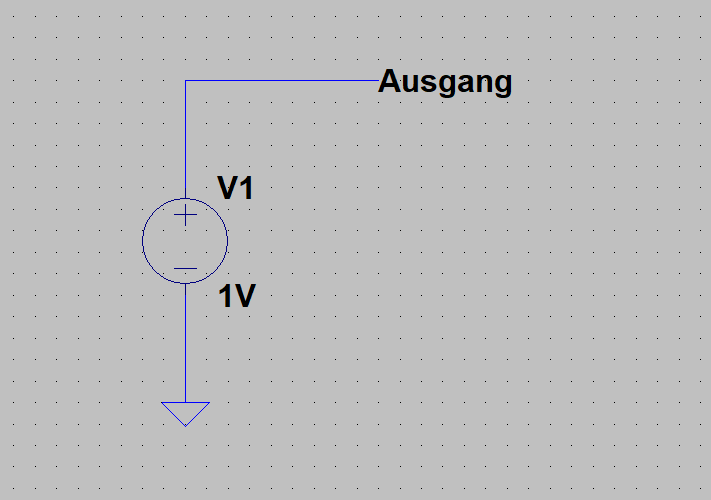
\includegraphics[scale=1]{21.PNG}
\caption{Darstellung einer Signalquelle in LTSpice}
\label{fig: Signalquelle}
\end{figure}
\newpage
Im Folgenden werden mit der Schaltung \fref{fig: Signalquelle}, verschieden Kurvenformen dargestellt und mit den jeweiligen Werten in LTSpice simuliert:



\subsection{Gleichspannungsquelle}
Folgender LTSpice Simulation und Graph wird durch eine Gleichspannungsquelle erzeugt.
\begin{figure}[ht!]
\centering
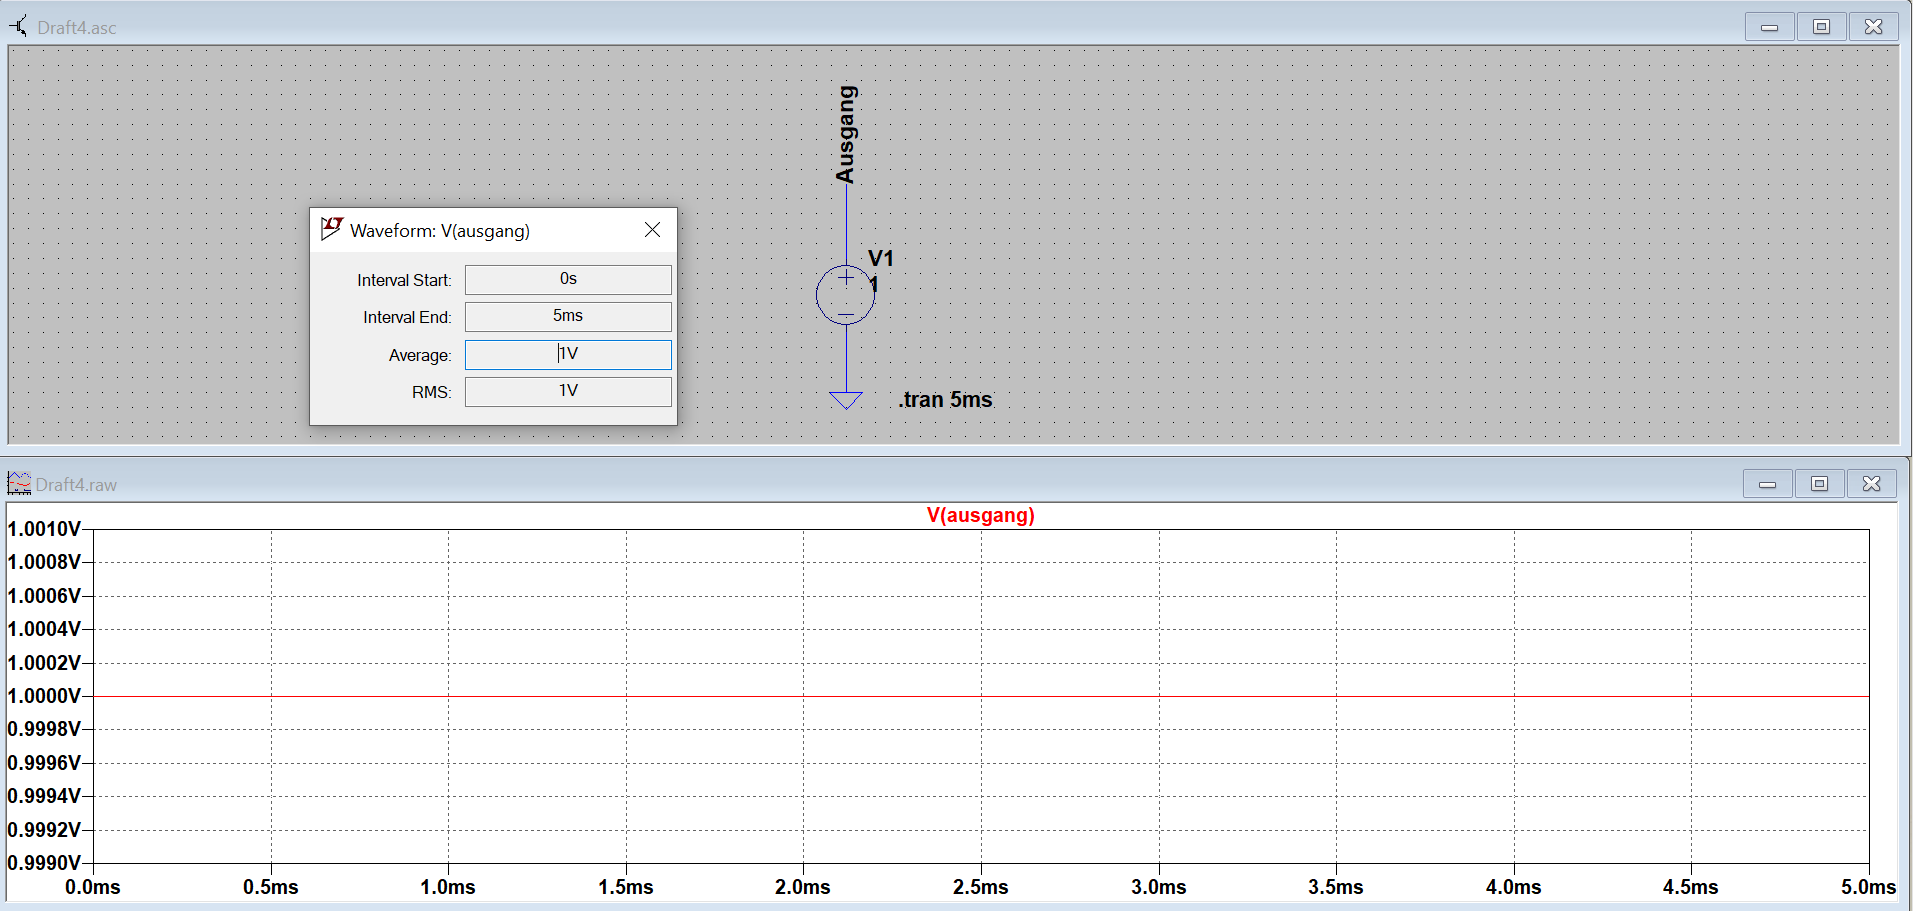
\includegraphics[scale=0.5]{211.PNG}
\caption{Gleichspannungsquelle $U=1V$}
\end{figure}

\subsection{Signussignal}
Um bei der folgenden Simulation ein richtiges Signal heraus zu bekommen, muss die $Periode(T)=1ms$ in die Frequenz f umgerechnet werden.
\begin{equation}
f=\frac{1}{T}=\frac{1}{10^{-3}}=1000Hz
\end{equation}
Folgender LTSpice Simulation und Graph wird durch die Werte erzeugt.
\begin{figure}[h!]
\centering
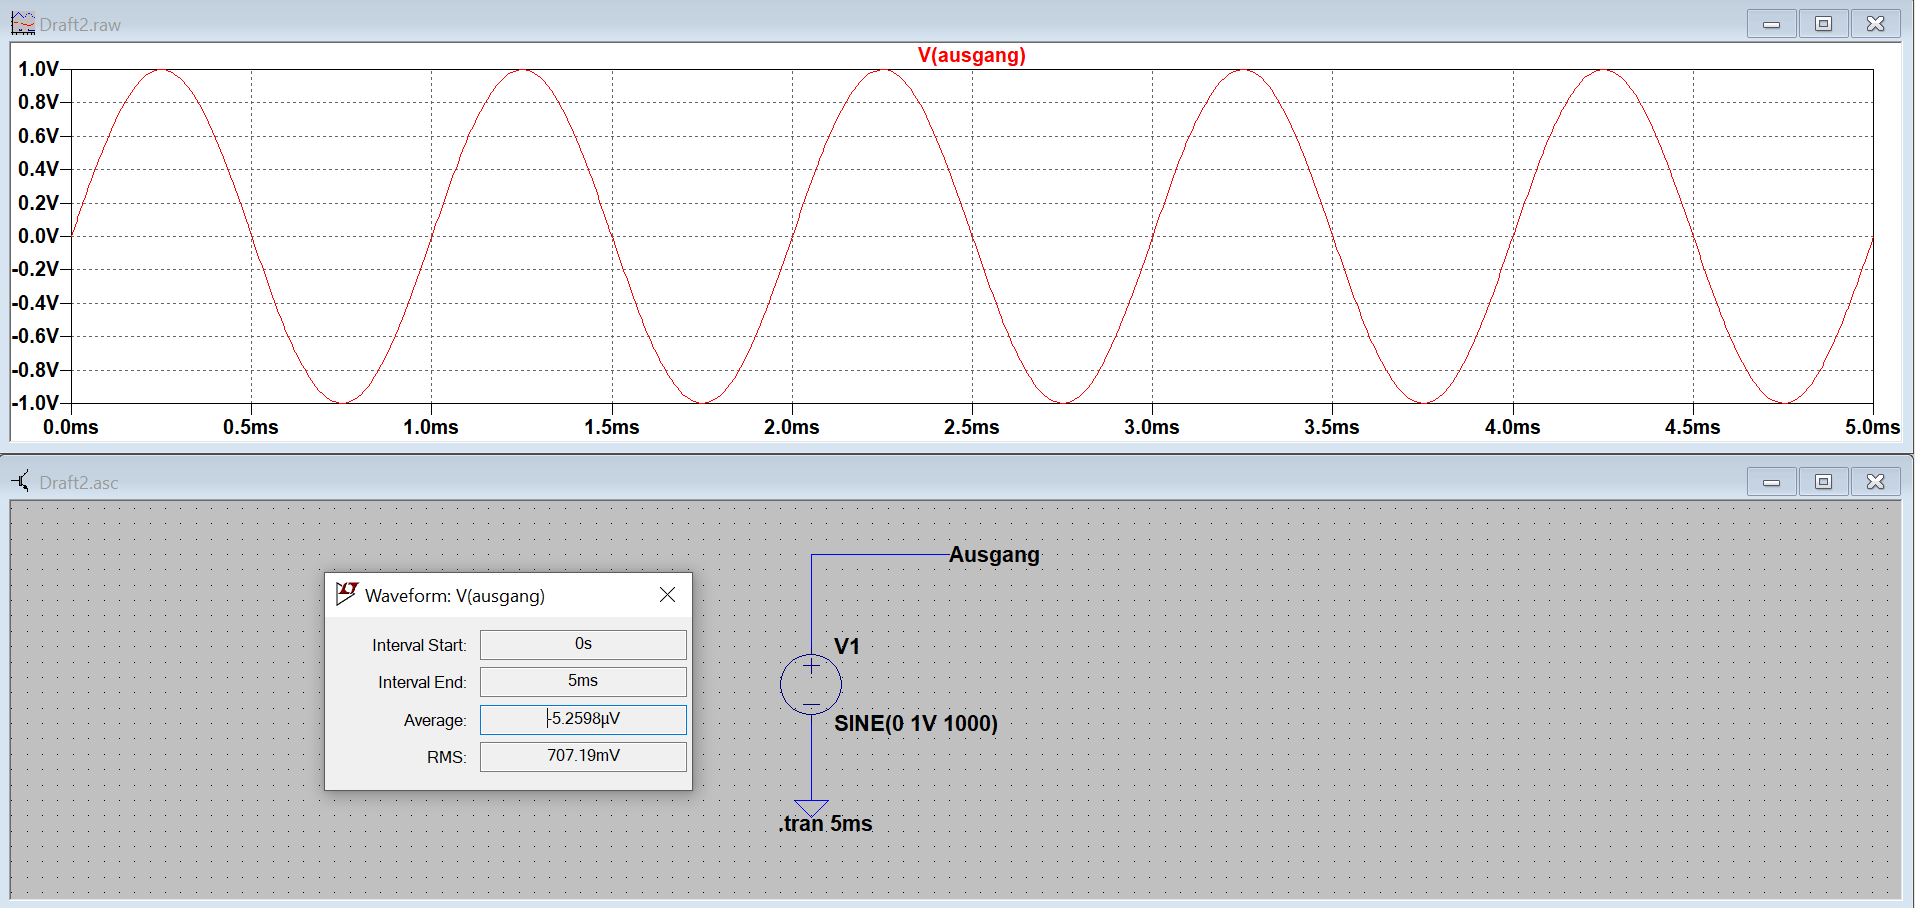
\includegraphics[scale=0.5]{212.PNG}
\caption{Sinussignal mit $\^{U}=1V$ und $T=1ms$}
\label{fig: Sinussignal}
\end{figure}
\newpage

\subsection{Symmetrisches Rechtecksignal}
Zum Darstellen eines symmetrischen Recktecksignals wird der $T_{rise}$ und $T_{fall}$ Wert angepasst. Dieser liegt in der Simulation bei jeweils 1ns. Die Spannungsquelle wird in den Pulse-Mode gestellt und die Werte für $\^{U}$,$T_{on}$ und f eingetragen \fref{fig: symRechtecksignal}. Dabei ergibt sich folgende LTSpice Simulation und Graph. 
\begin{figure}[ht!]
\centering
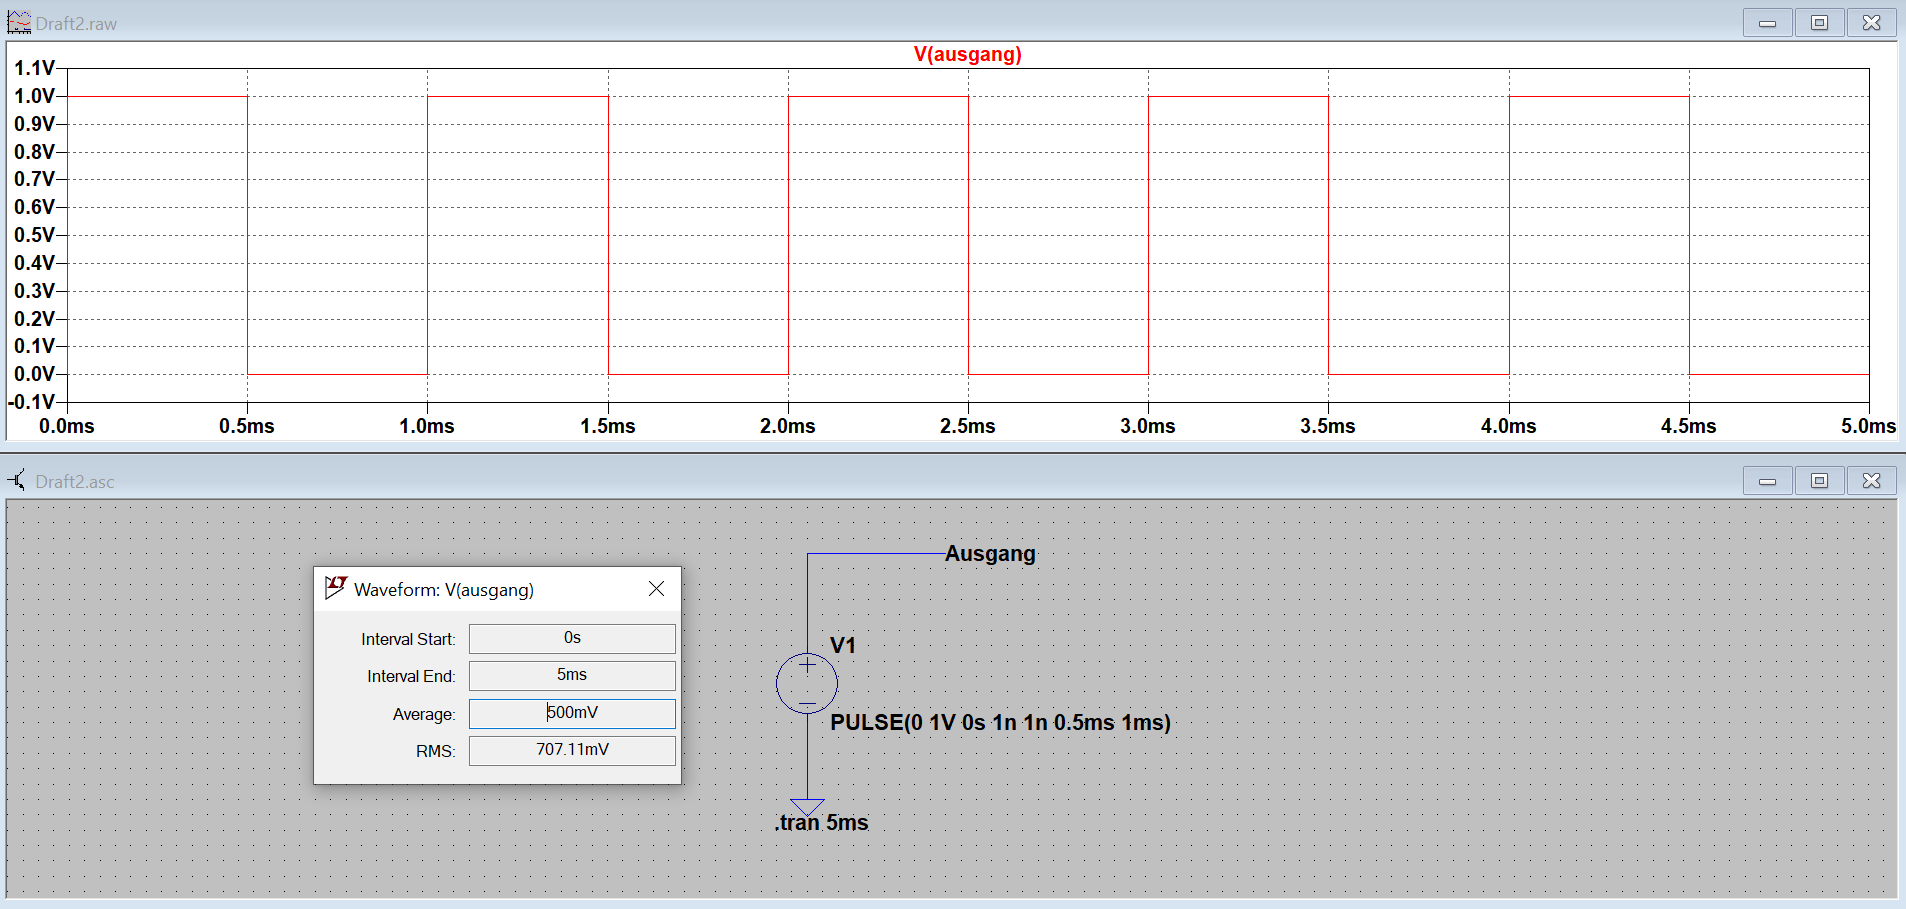
\includegraphics[scale=0.5]{213.PNG}
\caption{Symmetrisches Rechtecksignal mit $\^{U}=1V$, $T_{on}=0,5 ms$ und $f=1ms$}
\label{fig: symRechtecksignal}
\end{figure}

\subsection{Unsymmetrisches Rechtecksignal}
Zum Darstellen eines unsymmetrischen Recktecksignals wird ebenfalls der $T_{rise}$ und $T_{fall}$ Wert angepasst. Der liegt bei dieser Simulation bei jeweils 1ns. Durch eintragen der restlichen Werte \fref{fig: unsymRechtecksignal}, ergibt sich folgende LTSpice Simulation und Graph.
\begin{figure}[ht!]
\centering
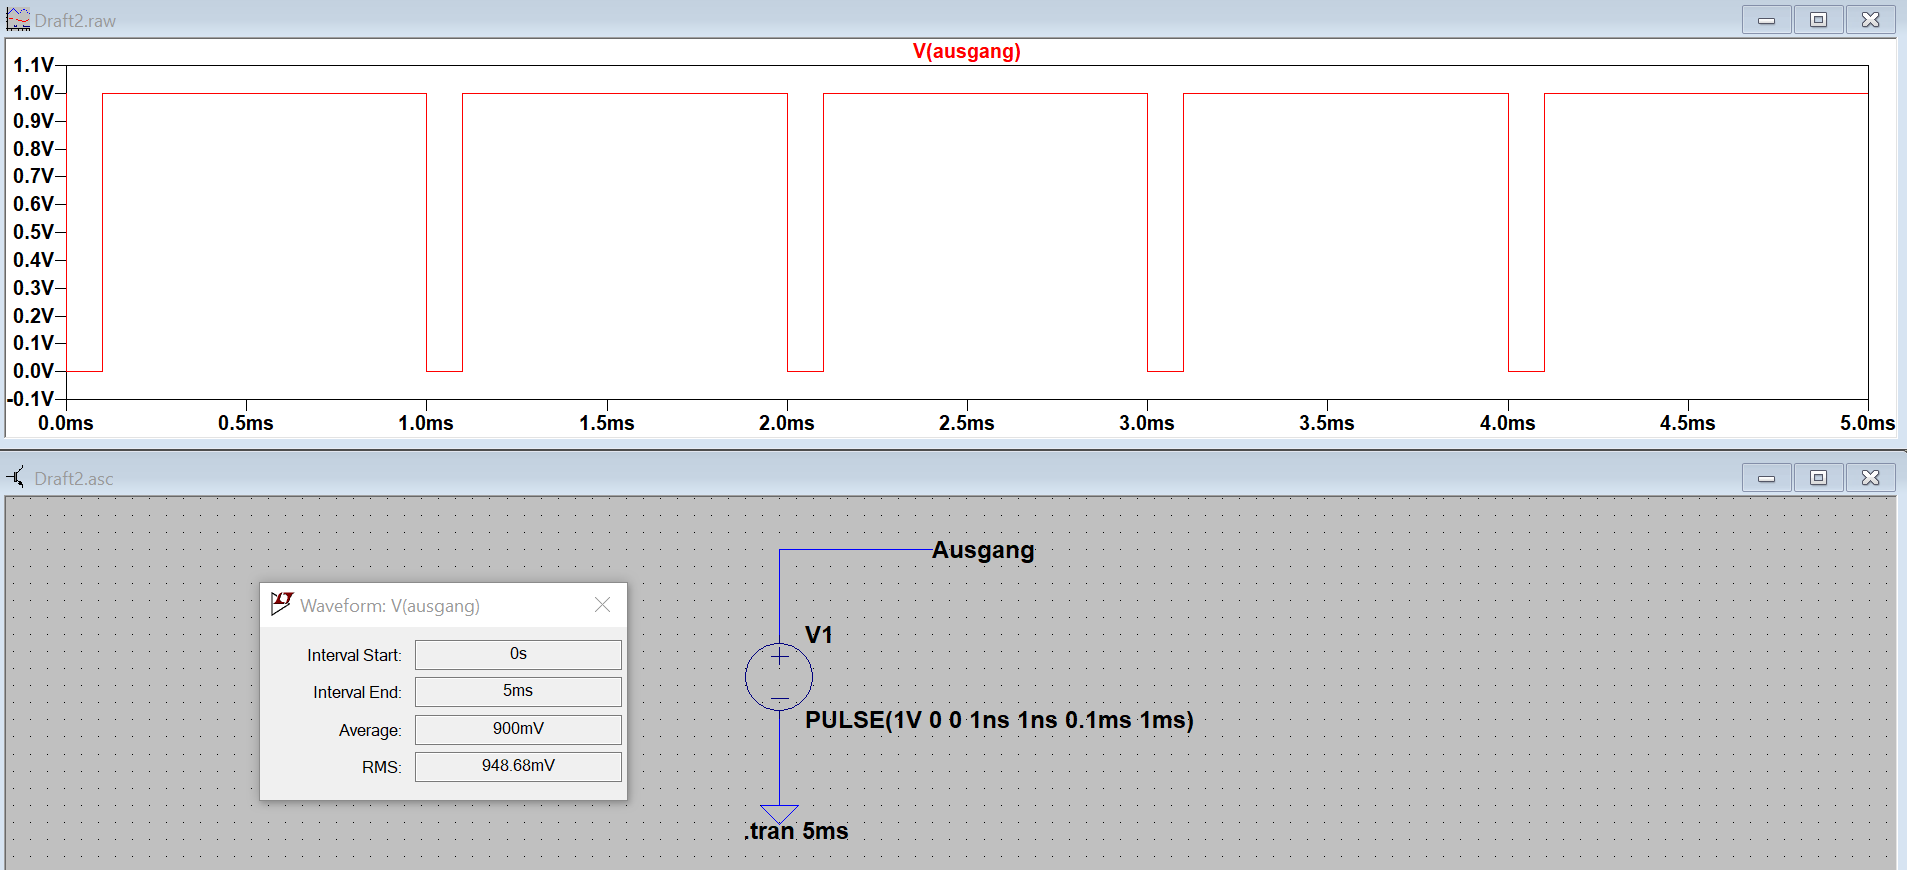
\includegraphics[scale=0.5]{214.PNG}
\caption{Unsymmetrisches Rechtecksignal mit $\^{U}=1V$, $T_{on}=0,1 ms$ und $f=1ms$}
\label{fig: unsymRechtecksignal}
\end{figure}

\subsection{Dreiecksignal}
Damit bei der Simulation mit LTSpice ein Dreiecksignal herauskommt, werden die Werte für $T_{rise}$, $T_{fall}$ und $T_{on}$ angepasst. 
$$T_{rise}=0.5ms$$
$$T_{fall}=0.5ms$$
$$T_{on}=0ms$$
Durch das einfügen der restlichen Werte \fref{fig: Dreiecksignal}, ergibt sich folgende LTSpice Simulation und Graph.
\begin{figure}[ht!]
\centering
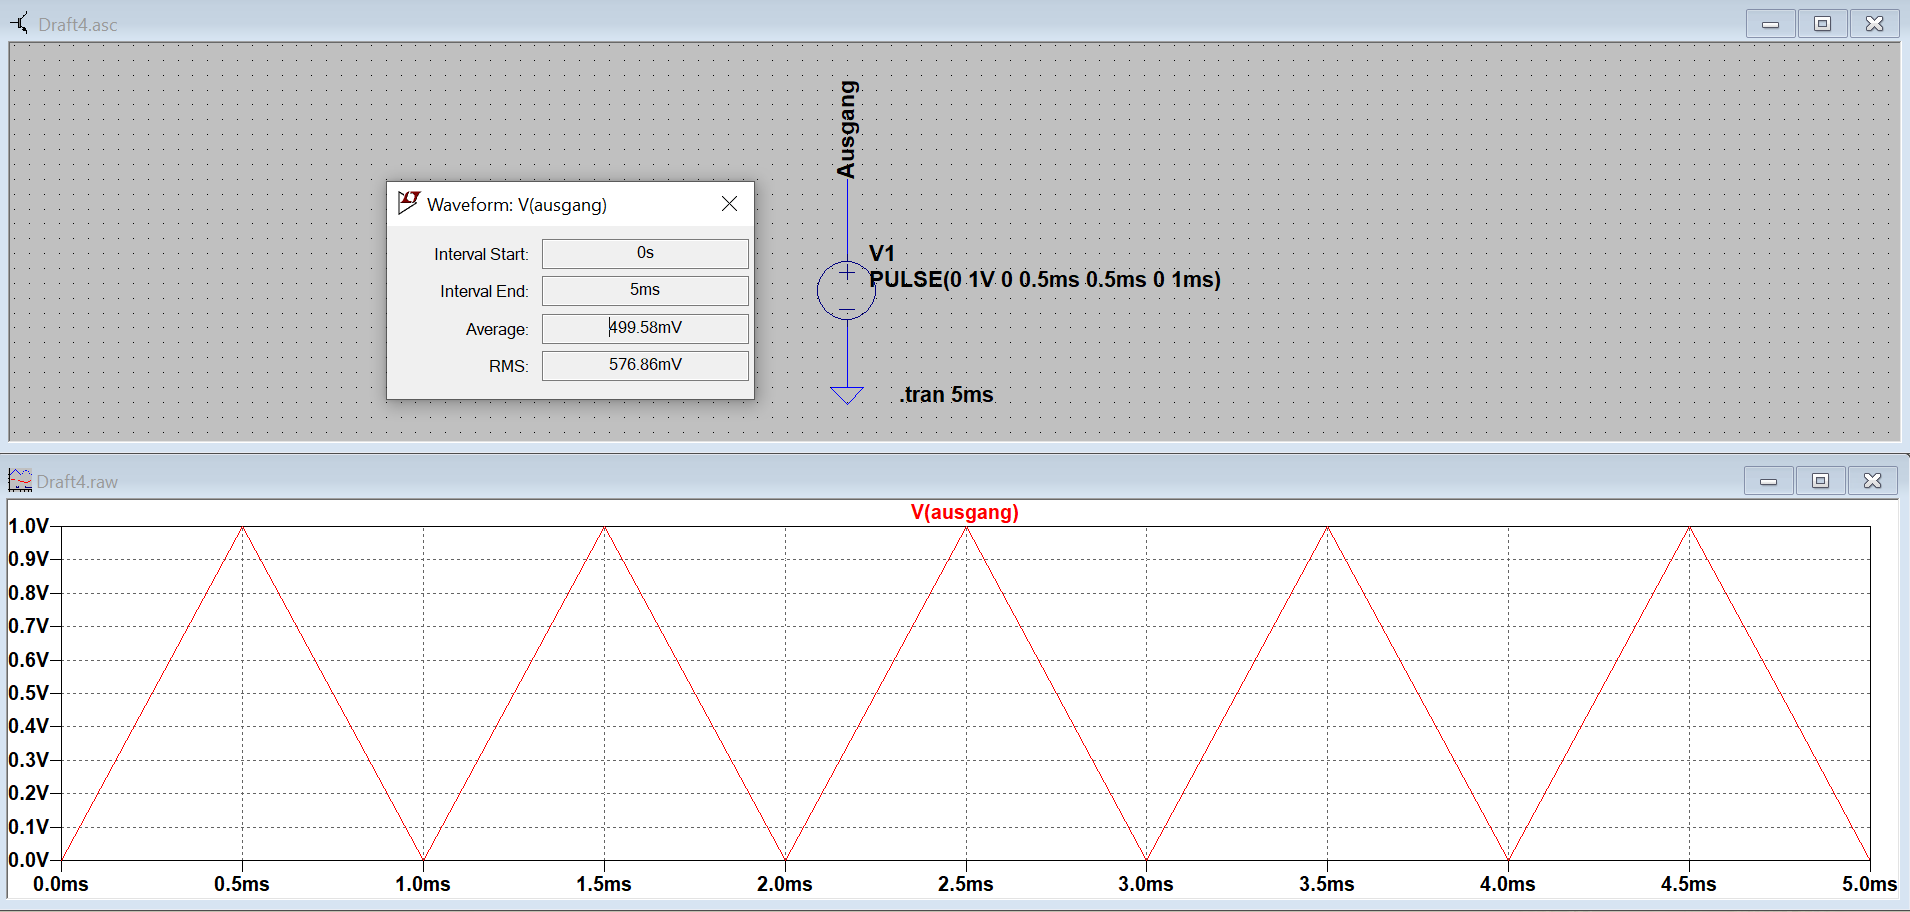
\includegraphics[scale=0.5]{215.PNG}
\caption{Dreiecksignal mit $\^{U}=1V$, $T=1ms$ }
\label{fig: Dreiecksignal}
\end{figure}
\newpage
\subsection{Sägezahnsignal}
Damit bei der Simulation mit LTSpice ein Dreiecksignal herauskommt, werden die Werte für $T_{rise}$, $T_{fall}$ und $T_{on}$ angepasst. 
$$T_{rise}=0.5ms$$
$$T_{fall}=1ns$$
$$T_{on}=0ms$$
Durch das einfügen der restlichen Werte \fref{fig: Sägezahnsignal}, ergibt sich folgende LTSpice Simulation und Graph.

\begin{figure}[ht!]
\centering
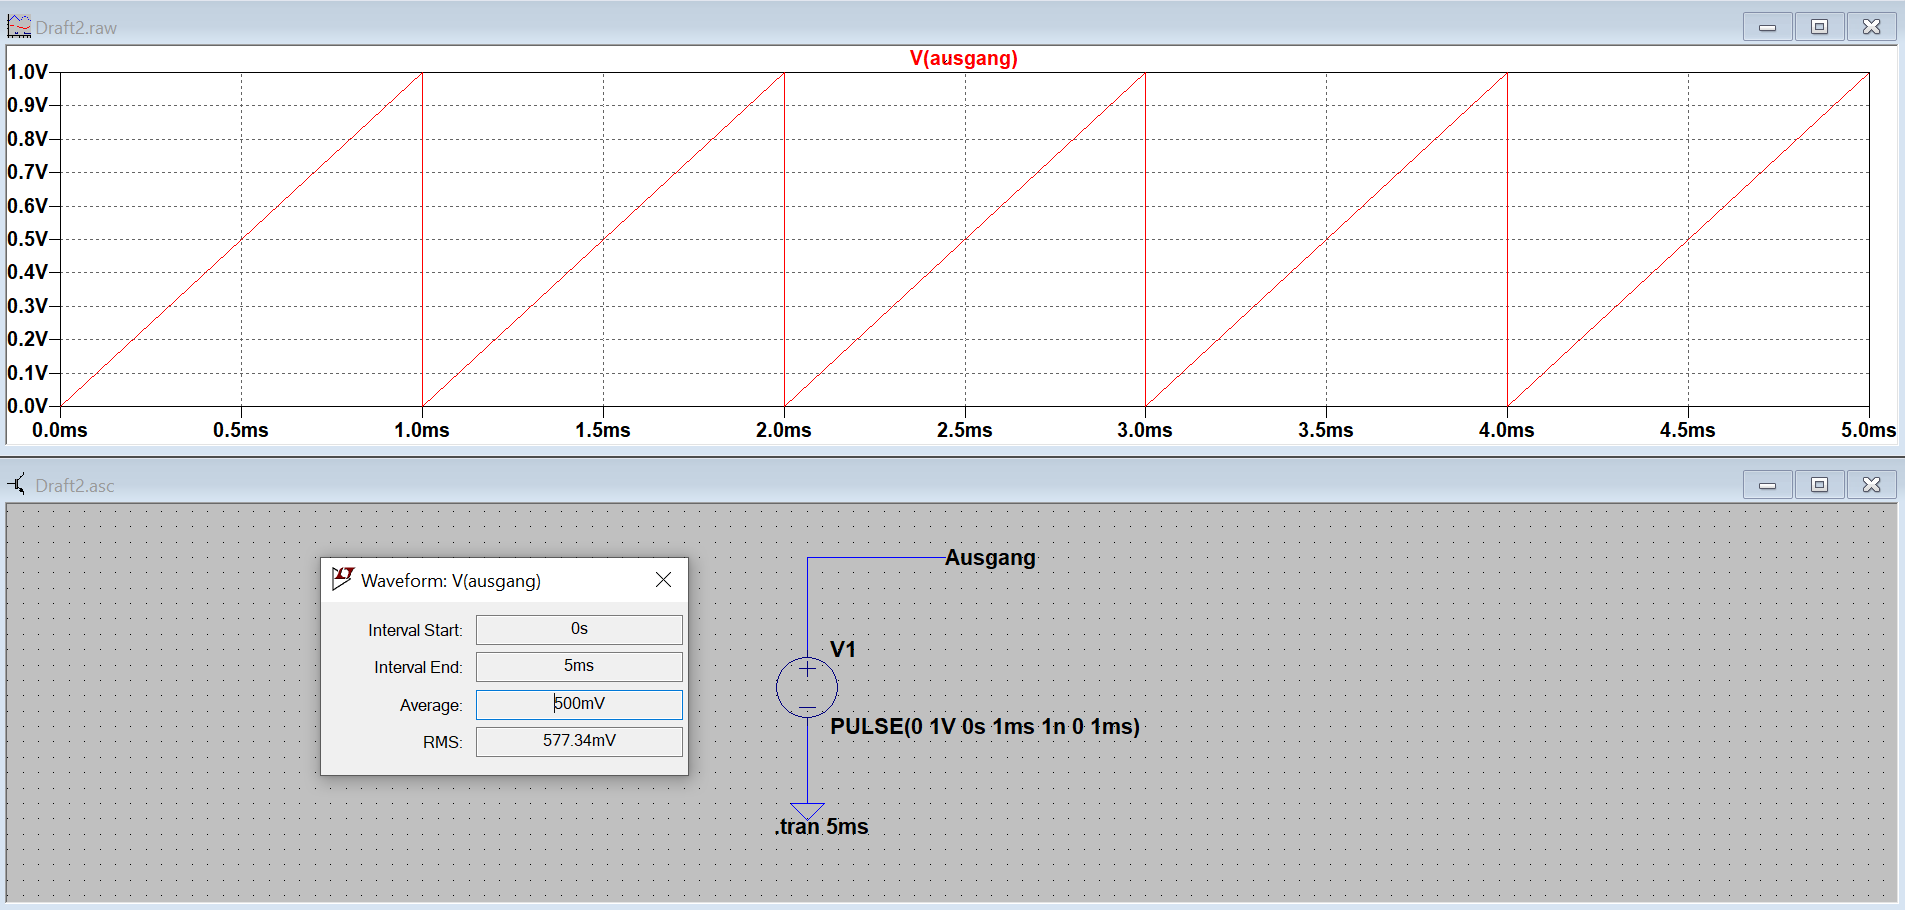
\includegraphics[scale=0.5]{216.PNG}
\caption{Sägezahnsignal mit $\^{U}=1V$, $T=1ms$}
\label{fig: Sägezahnsignal}
\end{figure}



Die von Hand ermittelten Effektivwerte (siehe Abschnitt 1.3) werden im Folgenden mit den Werten aus der Simulation verglichen. Die simulierten Effektivwerte sind auf den einzelnen Abbildungen \ref{fig: Signalquelle} bis \ref{fig: Sägezahnsignal} in den kleinen Kästchen unter RMS zu finden.
\begin{table}[ht!]
\centering
\caption{Wertetabelle für die Effektivwerte}
\label{fig: Effektivwerte}
\begin{tabular}{|c|c|c|} \hline
Signal & simulierte Effektivwerte & berechnete Effektiverte\\ \hline
Gleischspannungsquelle & 1V & 1V\\ \hline
Sinussignal & 707,19mV & 707mV\\ \hline
Symmetrisches Rechtecksignal & 707,11mV & 1V\\ \hline
Unsymmetrisches Rechtecksignal & 948,68mV & 1V\\ \hline
Dreiecksignal & 576,86mV & 578mV\\ \hline
Sägezahnsignal & 577,34mV & 578mV\\ \hline

\end{tabular}
\end{table}

Den Wert für das Sinussignal wurde in 1.3.1 Formel (1.9) berechnet. Der Wert für die Rechtecksignale sind in 1.3.2 Formel (1.17) und für die Dreiecksignale  in 1.3.3 Formel (1.26) zu finden. In Tab. \ref{fig: Effektivwerte} sind diese nochmal nebeneinander gestellt. Beim Vergleichen der Effektivwerte durch Berechnen und durch die Simulation ist direkt zu sehen, dass es dort kleine Unterschiede gibt. Bei dem Sinussignal und dem Dreiecksignal sind die Werte annäherungsweise gleich. Jedoch gibt es bei den Rechtecksignalen Unterschiede zwischen den Effektivwerten. Der des unsymmetrischen Dreiecksignals ist noch annäherungsweise an den errechneten 1V dran, der Effektivwert des symmetrischen Rechtecksignals hat jedoch einen Unterschied von fast 300mV. Dieser Wert passt eher zu dem berechneten Effektivwert des Sinussignals.

\newpage


\section{Spannungsteiler}
\subsection{Unbelasteter Spannungsteiler}
\begin{figure}[h!]
\centering
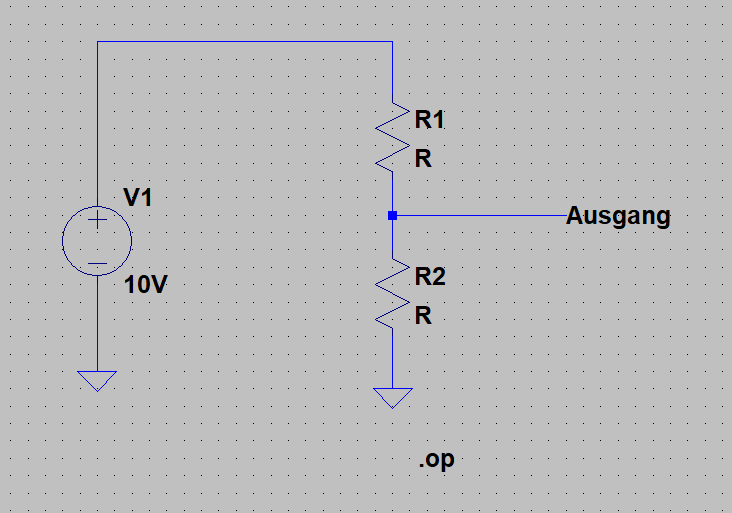
\includegraphics[scale=1]{221.PNG}
\caption{Unbelasteter Spannungsteiler}
\label{fig: Unbelasteter Spannungsteiler}
\end{figure}
Beim unbelasteten Spannungsteiler \fref{fig: Unbelasteter Spannungsteiler} werden jetzt die einzelnen Werte für $R_1$ und $R_2$ verändert und in die Schaltung eingegeben.

\begin{table}[h!]
\centering
\caption{Wertetabelle für den unbelasteten Spannungsteiler }
\label{fig: unbelasteter Spannungsteiler}
\begin{tabular}{|c|c|c|c|} \hline
$R_1$ in $\Omega$ & $R_2$ in $\Omega$ & $V_{aus}$ Simulation in V & $V_{aus}$ Spannungsteilerformel in V\\ \hline
$4,7k$ & $2,2k$ & 3,18841 & 3,18841\\ \hline
$47k$ & $22k$ & 3,18841 & 3,18841\\ \hline
$470k$ & $220k$ & 3,18841 & 3,18841\\ \hline
$4,7M$ & $2,2M$ & 3,18841 & 3,18841\\ \hline
$47M$ & $22M$ & 3,18841 & 3,18841\\ \hline

\end{tabular}
\end{table}

Mit der Spannungsteilerformel 
\begin{equation}
U_{aus}=U_{ges}\cdot \frac{R_2}{R_1+R_2}
\end{equation}
wird die Spannung am Ausgang von Hand berechnet. Dabei ist $U_{ges}=10V$, die Werte für $R_1$ und $R_2$ sind aus der Tabelle \ref{fig: unbelasteter Spannungsteiler} ablesbar.
Die Ergebnisse der Simulation und die Ergebnisse aus der Spannungsteilerformel sind identisch. Desweiteren sind die Ergebnisse für die verschiedenen Werte von $R_1$ und $R_2$ gleich, da diese Vielfache voneinander sind und sich somit die erhöhten Werte ausgleichen.

\subsection{Belasteter Spannungsteiler}
Der belastete Spannungsteiler ist wie der unbelastete Spannungsteiler aufgebaut, jedoch wird an den Ausgang ein Innenwiderstand von $R_3=10M\Omega$ dazugeschaltet. Dies ist in Abb.\ref{fig: bel.Spannungsteiler} veranschaulicht.
\begin{figure}[h!]
\centering
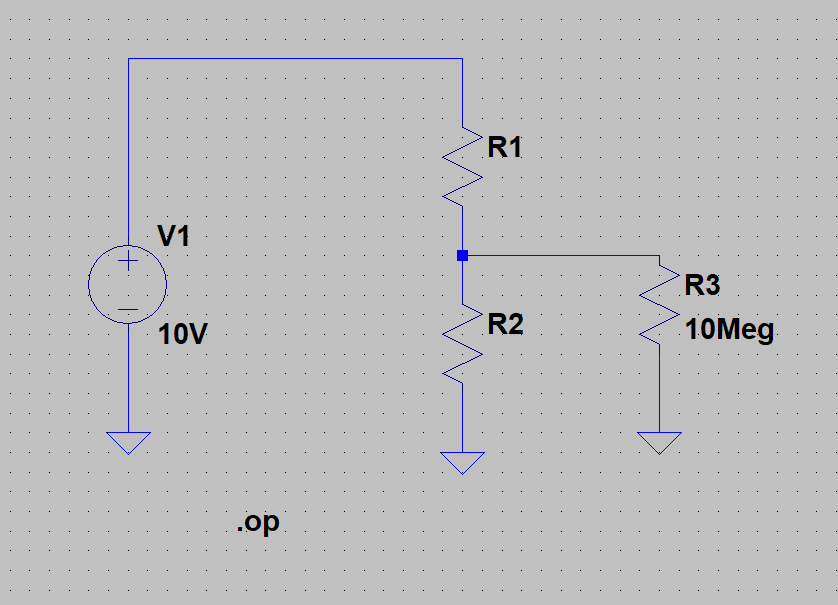
\includegraphics[scale=1]{222.PNG}
\caption{Belasteter Spannungsteiler}
\label{fig: bel.Spannungsteiler}
\end{figure}

\begin{table}[h!]
\centering
\caption{Wertetabelle für den unbelasteten Spannungsteiler }
\label{fig: belasteter Spannungsteiler}
\begin{tabular}{|c|c|c|} \hline
$R_1$ in $\Omega$ & $R_2$ in $\Omega$ & $V_{aus}$ Simulation in V \\ \hline
$4,7k$ & $2,2k$ & 3.18793\\ \hline
$47k$ & $22k$ & 3.18363\\ \hline
$470k$ & $220k$ & 3.14133\\ \hline
$4,7M$ & $2,2M$ & 2.77288\\ \hline
$47M$ & $22M$ & 1.2761\\ \hline

\end{tabular}
\end{table}

Beim Vergleichen der Ausgangsspannung $V_{aus}$ der Simulation (siehe Tab.~\ref{fig: belasteter Spannungsteiler} und~\ref{fig: unbelasteter Spannungsteiler})fällt auf das die Werte voneinander abweichen. Das liegt daran, das ein nicht variabler Widerstand $R_3=10M\Omega$ (Innenwiderstand des Voltmeters) parallel zu $R_2$ dazugeschaltet ist. Da dieser immer den gleichen Wert besitzt, jedoch die Werte für $R_1$ und $R_2$ steigen, verändert sich auch die Spannung am Ausgang. Dies  ist auch an der Formel für einen belasteten Spannungsteiler zu sehen.
\begin{equation}
U_{aus}=U_{ges}\cdot \frac{R_2||R_3}{R_1+(R_2||R_3)}
\end{equation}
Hier wird der Widerstand $R_3$ parallel zu $R_2$ geschaltet und  mit dem festen Wert für $R_3$ gerechnet. Dadurch sinkt die Spannung bei höheren Widerstandswerten von $R_1$ und $R_2$.

\section{Potentiometer}
\begin{figure}[h!]
\centering
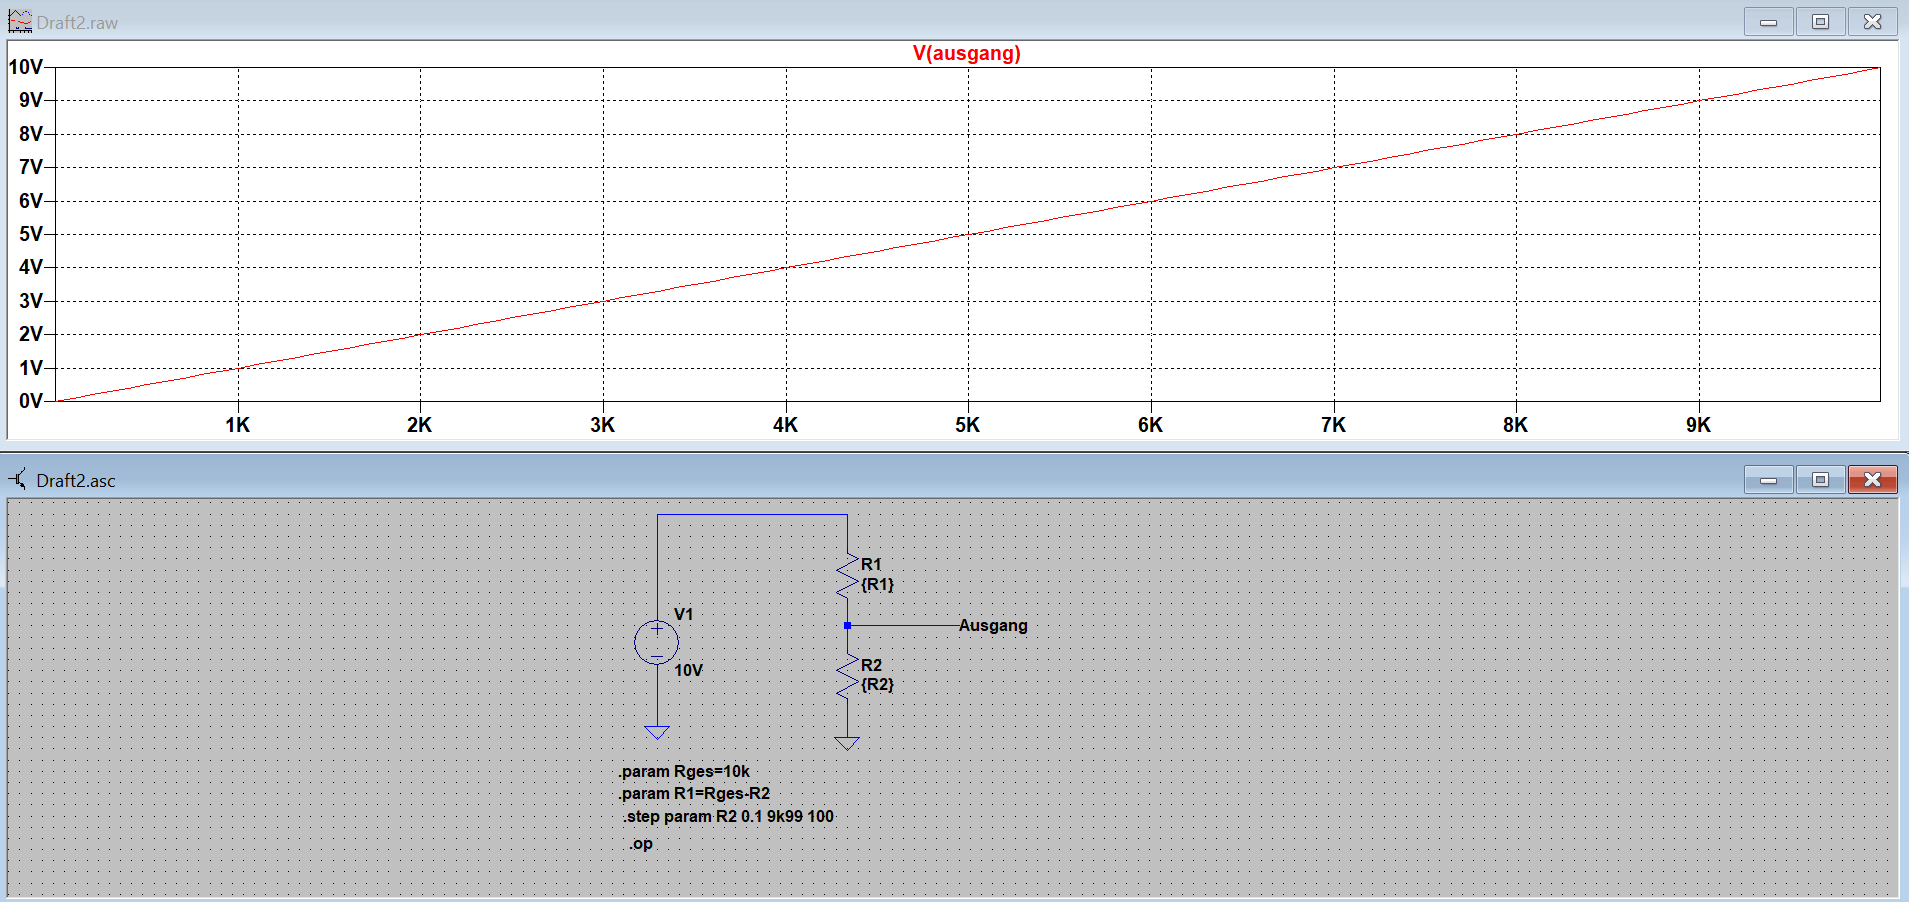
\includegraphics[scale=0.5]{23.PNG}
\caption{Darstellung eines Potentiometers}
\label{fig: Potentiometer}
\end{figure}

Die Schaltung in Abb.~\ref{fig: Potentiometer} sieht aus wie die Abb.~\ref{fig: Unbelasteter Spannungsteiler} eines unbelasteten Spannungsteilers. Jedoch ist beim Potentiometer der Widerstand $R_1$ vom Widerstand $R_2$ abhängig.
\begin{equation}
R_1=R_{ges}-R_2
\end{equation}
Die Werte von $R_2$ ändern sich dabei in $100\Omega$ Schritten im Intervall von $0.1\Omega$ bis $9k99\Omega$, unter der Bedingung:
$$0\Omega \leq R_2\leq R_{ges}$$
Die Simulation beginnt mit $0.1\Omega$ und endet mit $9k99\Omega$ damit $R_1$ nicht $0\Omega$ wird.\\
Im Graphen \fref{fig: Potentiometer} ist zu sehen, das mit steigendem $R_2$ auch die Ausgangsspannung $V_{aus}$ steigt.








    \chapter{Versuchsdurchführung}
    \section{Arbeitsgerade am Transformator in der Reihenschaltung}  
         
        Zunächst haben wir den Lastwiderstand in Reihe  zum Transformator geschalten \figref{fig:reihenschaltung}. Hier wurde der Lastwiderstand in gewissen Schritten verändert, dabie ändert ich die Spannung $U_{sek}$.
        Im Anschluss wird der Strom $I_{sek}$ errechnet. Die Werte für den Lastwiderstand werden von $12\,\ohm$ auf $22\,\ohm$ um jeweils $2\,\ohm$ erhöht.
        Die Werte wurden in einer Tabelle zusammengetragen \tabref{tab:reihenschaltung}.
        \begin{equation}
            I_{sek}=\frac{U_{sek}}{I_{sek}}
        \end{equation}

        
            \begin{table}[ht!]
                \centering
                \caption{Messwerte zur Reihenschaltung}
                \label{tab:reihenschaltung}
                \begin{tabular}{|c|c|c|}
                    \hline
                    $R_{Last}$ in $\ohm$& $U_{sek}$ in $V$& $I_{sek}$ in $A$\\
                    \hline
                        12 & 18,114 & 1,510\\
                        14 & 18,661 & 1,333\\
                        16 & 19,002 & 1,188\\
                        18 & 19,318 & 1,073\\
                        20 & 19,578 & 0,979\\
                        22 & 19,797 & 0,900\\
                    \hline
                \end{tabular} 
            \end{table}
        Die Auswertung der gemessenen und errechneten Daten wurden mit der Software SciDAVis realisiert \fref{fig:reihenschaltung_aus}. 
        
        \begin{figure}[ht!]
            \centering
            \includegraphics[width=.9\textwidth]{Bilder/u_i_diagramm_reihenschaltung.PNG}
            \caption{Auswertung der Messwerte in der Reihenschaltung}
            \label{fig:reihenschaltung_aus}
        \end{figure}

        Durch die Auswertung mit der linearen Anpassung ergab sich eine Geradengleichung wie folgt.
        \begin{equation}
            U(I)= -2,719\,\ohm\cdot I + 22,244\, V
        \end{equation}
        Dabei ergibt sich eine Leerlaufspannung von
        \begin{equation}
            U_0 = U_{sek}(0\, A) = 22,244\, V 
        \end{equation}
        und ein Kurzschlussstrom von 
        \begin{equation}
            U_{sek}(I_{sek})\overset{!}{=} 0\,\Rightarrow\, I_k = \frac{22,244\, V}{2,719\,\ohm}= 8,181\, A
        \end{equation}
        Die Steigung der Geradengleichung gibt hier den durchschnittlichen Innenwiderstand. Dieser beträgt $2,719\,\ohm$.

    \section{Arbeitsgerade am Transformator in der Parallelschaltung} 
        Im Anschluss wurde das gleiche mit der Parallelschaltung durchgeführt\figref{fig:parallelschaltung}. Hier war der Wertebereich des Lastwiderstands zwischen $4\,\ohm$ und $14\,\ohm$. Auch diese Werte wurden in einer Tabelle zusammengetragen \tabref{tab:parallelschaltung}
        \begin{table}[ht!]
            \centering
            \caption{Messwerte zur Parallelschaltung}
            \label{tab:parallelschaltung}
            \begin{tabular}{|c|c|c|}
                \hline
                $R_{Last}$ in $\ohm$& $U_{sek}$ in $V$& $I_{sek}$ in $A$\\
                \hline
                    4 & 9,502 & 2,375\\
                    6 & 9,991 & 1,665\\
                    8 & 10,256 & 1,282\\
                    10 & 10,421 & 1,042\\
                    12 & 10,534 & 0,878\\
                    14 & 10,617 & 0,758\\
                \hline
            \end{tabular} 
        \end{table}
        Die Werte wurden ebenfalls mit der Software SciDAVis ausgewertet \fref{fig:parallelschaltung_aus}


        \begin{figure}[ht!]
            \centering
            \includegraphics[width=.9\textwidth]{Bilder/u_i_diagramm_parallelschaltung.PNG}
            \caption{Auswertung der Messwerte in der Parallelschaltung}
            \label{fig:parallelschaltung_aus}
        \end{figure}

    
        Auch hier wurde mit Hilfe der linearen Anpassung die Geradengleichung aufgestellt, diese wie folgt lautet.
        \begin{equation}
            U(I)= -0,690\,\ohm\cdot I + 11,140\, V
        \end{equation}
        Dabei ergibt sich eine Leerlaufspannung von
        \begin{equation}
            U_0 = U_{sek}(0\, A) = 11,140\, V 
        \end{equation}
        und ein Kurzschlussstrom von 
        \begin{equation}
            U_{sek}(I_{sek})\overset{!}{=} 0\,\Rightarrow\, I_k = \frac{11,140\, V}{0,690\,\ohm}= 16,145\, A
        \end{equation}
        Auch hier gibt die Steigung der Geradengleichung den durchschnittlichen Innenwiderstand an. Dieser beträgt $0,690\,\ohm$.
    \newpage
    
    \section{Brückengleichrichter mit Glättungskondensator}
        In der nächsten Aufgabe wurde der Brückengleichrichter \figref{fig:gleichrichter} in LTSpice mit einem nicht geladenen Konensator simuliert.
        Die wurde ermöglicht in dem man die Simulation in den ersten $100\, ms$ betrachtet \fref{fig:unaufgeladenner_kondensator}

        \begin{figure}[ht!]
            \centering
            \includegraphics[width=.9\textwidth]{Bilder/unaufgeladenner_kondensator.png}
            \caption{Simulationskurven mit nicht geladenen Kondensator}
            \label{fig:unaufgeladenner_kondensator}
        \end{figure}

        Um ein eingeschwungenes Schaltbild zu erzeugen wird die Simulation mit einem Offset von $0,9\, s$ für $100\, ms$ gestartet.

        \begin{figure}[ht!]
            \centering
            \includegraphics[width=.9\textwidth]{Bilder/aufgeladenner_kondensator.png}
            \caption{Simulationskurven mit eladenen Kondensator}
            \label{fig:aufgeladenner_kondensator}
        \end{figure}

    \newpage
    \section{Wirkungsgrad}
        Für die Ermittlung des Wirkungsgrades wird die Schaltung aus der vorherigen Aufgabe angepasst \fref{fig:schaltbild_wirkungsgrad}.
        Die Änderung die vorgenommen wird ist beim Laststrom. Dieser wird auf $1\, A$ geändert.\par
        \begin{figure}[ht!]
            \centering
            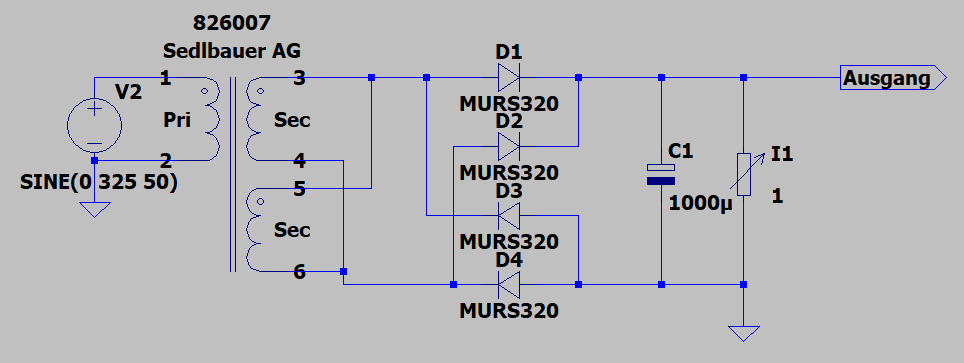
\includegraphics[width=.9\textwidth]{Bilder/wirkungsgrad.png}
            \caption{Schaltbild für die Simulation und Auswertung des Wirkungsgrades}
            \label{fig:schaltbild_wirkungsgrad}
        \end{figure}

        Die Leistung der einzelnen Bauteile wird aus LTSpice abgelesen. 
        \begin{center}
            \begin{tabular}{l r}
                \hline
                Bauteile & Leistung \\
                \hline
                $\overset{-}{P}_{Prim}$& $10,436\, W$ \\
                $\overset{-}{P}_{Last}$ & $-16,852\, W$ \\
                $\overset{-}{P}_{D_1}=\overset{-}{P}_{D_4}$ & $389,87\, mW$\\
                $\overset{-}{P}_{D_2}=\overset{-}{P}_{D_3}$ & $392,92\, mW$\\
                $\overset{-}{P}_{C_1}$ & $-36,759\, mW$\\
                $\overset{-}{P}_{sek}$ & $4,883\, W$\\
                \hline
            \end{tabular} 
        \end{center}

        Setzt man nun die mittlere Leistung des Lastwiderstand $\overset{-}{P}_{Last}$ und der Spannungsquelle $\overset{-}{P}_{Prim}$ in die Gleichung für die berechnung des Wirkungsgrads, so erhält man 

        \begin{equation}
            \mu=\frac{P_{Nutz}}{P_{Aufwand}}= \frac{\overset{-}{P}_{Last}}{\overset{-}{P}_{Prim}}= \frac{10,436\, W}{16,852\, W}= 0,619 = 61,9\%
        \end{equation}

        Wenn man alle Einzelleistungen aufsummiert, exklusive der Primärspulenleistung, ergibt sich: 
        \begin{equation}
            \overset{-}{P}_{Last}+2\cdot\overset{-}{P}_{D_1}+2\cdot\overset{-}{P}_{D_2}+\overset{-}{P}_{C_1}+\overset{-}{P}_{sek}= \overset{-}{P}_{alle}
        \end{equation}

        \begin{equation}
            10,436\, W+2\cdot 389,87\, mW+2\cdot 392,92\, mW + 36,759\, mW + 4,883\, W = 16,139\, W 
        \end{equation}
        Das Ergebnis ist ungefähr der Primärleistung und die logische Konsequenz des addierens aller Teilleistungen.



    
    
    %\printbibliography
\end{document}